\documentclass{article}

\usepackage{tikz}
\usetikzlibrary{shapes,arrows}
\begin{document}

\centering
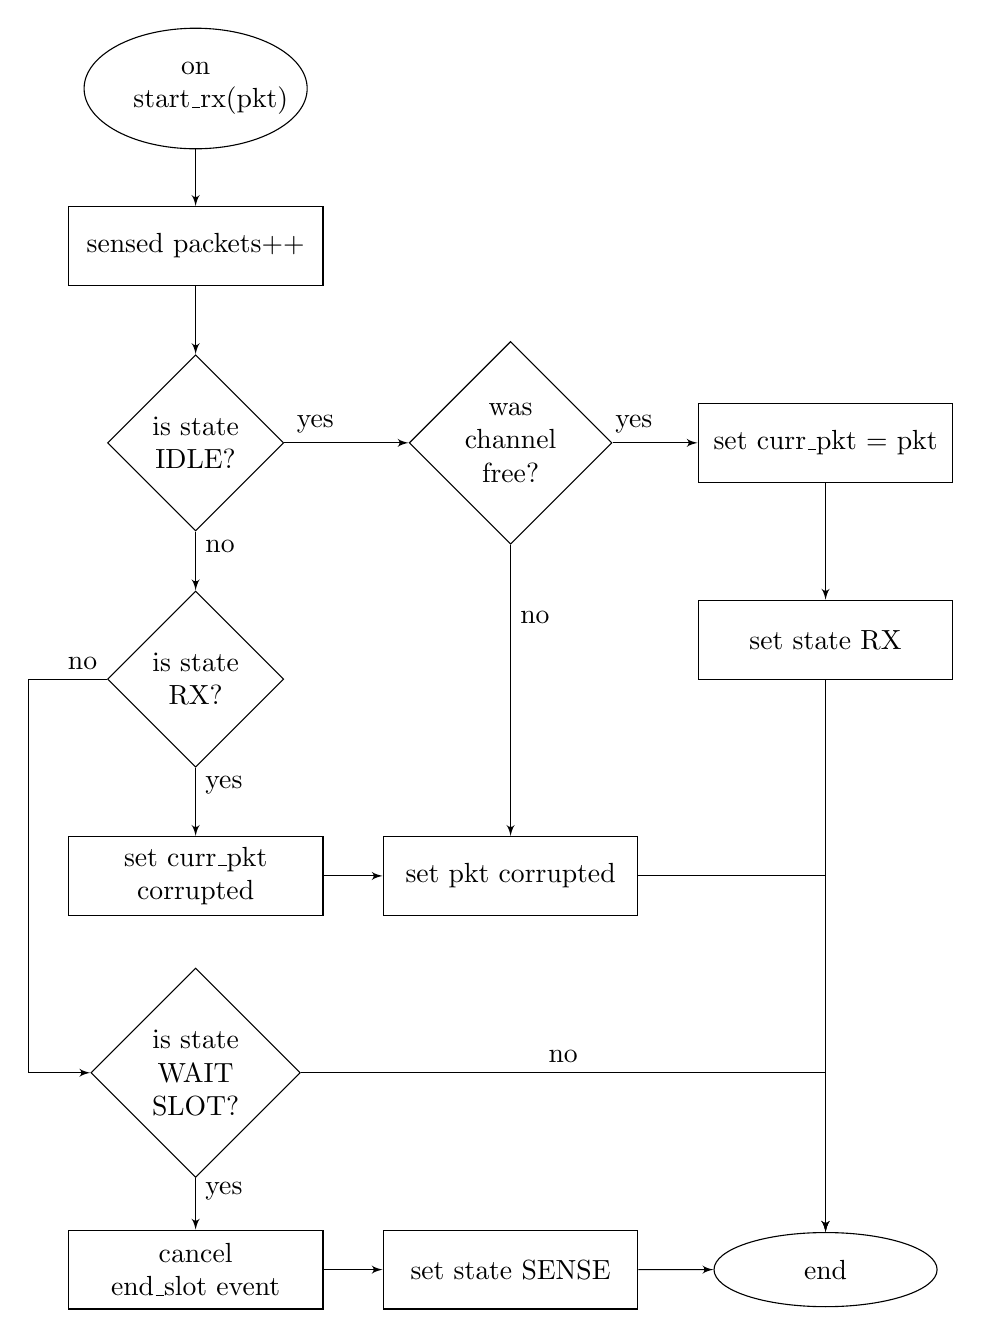
\begin{tikzpicture}[node distance = 1.5cm, auto]
    \tikzstyle{terminator} = [ellipse, draw,
    text width=4.5em, text centered, inner sep=6pt]
  \tikzstyle{decision} = [diamond, draw,
    text width=4.5em, text centered, node distance=3cm, inner sep=0pt]
  \tikzstyle{block} = [rectangle, draw, text width=3cm, text centered, minimum width=3cm,
    minimum height=1cm]
  \tikzstyle{line} = [draw, -latex']

  % Place nodes
  \node [terminator] (init) {on start\_rx(pkt)};
    \node [block, below of=init, node distance=2cm] (addrcv) {sensed
    packets++ };
  \node [decision, below of=addrcv, node distance=2.5cm] (idle) {is state
    IDLE?};
  \node [decision, below of=idle, node distance=3cm] (rx) {is state
    RX?};
    \node [decision, right of=idle, node distance=4cm] (count) {was
      channel free?};
  \node [block, right of=count, node distance=4cm] (setcurr) {set
    curr\_pkt = pkt};
  \node [block, below of=setcurr, node distance=2.5cm] (setrx) {set
    state RX};

  \node [block, below of=rx, node distance=2.5cm] (coll) {set
      curr\_pkt corrupted};
  \node [block, right of=coll, node distance=4cm] (corr) {set pkt
     corrupted};

  \node [decision, below of=coll, node distance=2.5cm] (slot) {is state
      WAIT SLOT?};
  \node [block, below of=slot, node distance=2.5cm] (cancslot) {cancel
    end\_slot event};
  \node [block, right of=cancslot, node distance=4cm] (setsense) {set
    state SENSE};
  \node [terminator, below of=setrx, node distance=8cm] (end) {end};

  % Draw edges
  \path [line] (init) -- (addrcv);
  \path [line] (addrcv) -- (idle);

  \path [line] (idle) -- node [near start] {yes} (count);
  \path [line] (idle) -- node [near start] {no} (rx);
  \path [line] (count) -- node [near start] {yes} (setcurr);
  \path [line] (count) -- node [near start] {no} (corr);
  \path [line] (corr) -| (end);
  \path [line] (setcurr) -- (setrx);
  \path [line] (setrx) -- (end);
  \path [line] (rx) -- node [near start] {yes} (coll);
  \path [line] (coll) -- (corr);
  \path [line] (slot) -- node [near start] {yes} (cancslot);
  \path [line] (cancslot) -- (setsense);
  \path [line] (slot.east) -| node [near start] {no} (end);
  \path [line] (setsense) -- (end);
  \path [line] (rx.west) |- node [near start, anchor=south east] {no} ++(-1cm,0) |- (slot);

\end{tikzpicture}

\end{document}
